\subsection{Metrics to Quantify Differential Expression}

\begin{figure}
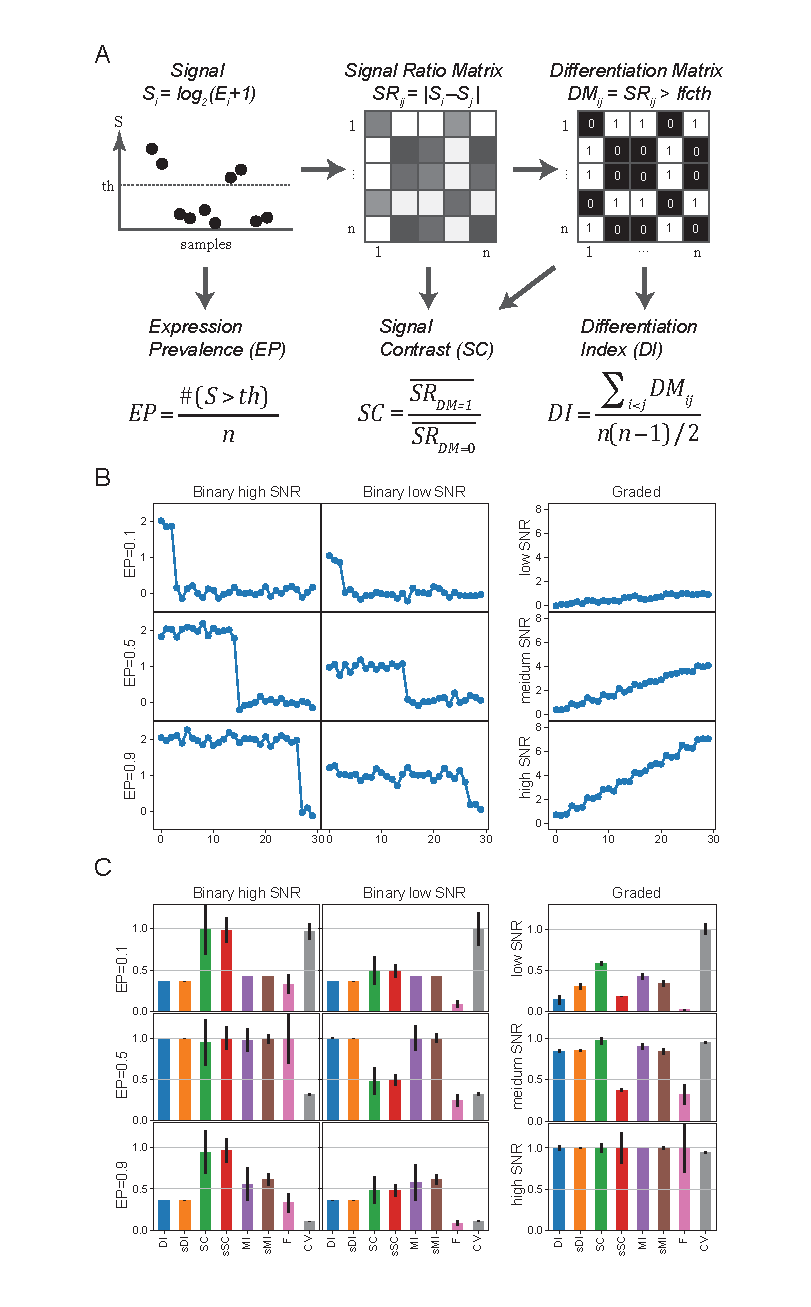
\includegraphics[width=0.87\linewidth]{Fig-metrics-v2}
\caption{Metrics to Quantify Expression Diversity.
\textbf{(A)} Definition of EP,SC and DI.
\textbf{(B)} Example expression patterns. For both binary and graded, expression values for 30 samples (10 groups with 3 replicates) with noise level of 0.1 are generated. Noises are sampled from Gaussian distribution. For binary patterns, EP of 0.1,0.5,0.9, and SNR of 20 (high SNR) and 10 (low SNR) are generated. For graded patterns, successive groups are separated by 0.1 (low SNR), 0.4 (medium SNR) and 0.7 (high SNR).
\textbf{(C)} Metrics corresponding to example patterns shown in (B). MI:mutual information, F:ANOVA F-value, CV:coefficient of variation. Prefix s (for sDI and sMI) indicates that sample label instead of group label is used (i.e. treated as unlabeled, no replicate). Values are average of 100 trials and normalized by the maximum within each metric. Error bars represent standard deviations. 
}